\documentclass[sigplan,review,anonymous]{acmart}

% EuroSys 2027 fall-cycle submission draft.
% The official CFP encourages the ACM SIGPLAN template, requires double-blind
% review, page numbers, and at most 12 pages of technical content.
\acmSubmissionID{PAPER-ID}
\setcopyright{none}
\settopmatter{printfolios=true,printacmref=false,printccs=false}
\renewcommand\footnotetextcopyrightpermission[1]{}
\pagestyle{plain}
\acmConference[EuroSys '27]{The European Conference on Computer Systems}{April 19--23, 2027}{Rabat, Morocco}
\acmYear{2027}
\copyrightyear{2027}
\acmDOI{}
\acmISBN{}

\usepackage{amsmath}
\usepackage{mathtools}
\usepackage{booktabs}
\usepackage{tabularx}
\usepackage{multirow}
\usepackage{array}
\usepackage{enumitem}
\usepackage{xspace}
\usepackage{balance}
\usepackage{algorithm}
\usepackage[noend]{algpseudocode}
\usepackage{tikz}
\usetikzlibrary{arrows.meta,positioning,fit,calc,shapes.geometric,patterns}
\usepackage{pgfplots}
\pgfplotsset{compat=1.18}
\usepackage{microtype}
\usepackage{cleveref}

\input{rai_results}

\newcommand{\sys}{\textsc{RAI}\xspace}
\newcommand{\Slot}{\mathsf{Slot}}
\newcommand{\Cut}{\mathsf{CloseCut}}
\newcommand{\Record}{\mathsf{CloseRecord}}
\newcommand{\hash}{\mathsf{H}}
\newcommand{\timeout}{\mathsf{timeout}}
\newcommand{\finalized}{\mathsf{finalized}}
\newcommand{\released}{\mathsf{released}}
\newcommand{\canon}{\mathsf{canon}}
\newcommand{\committee}{\mathcal{Q}}
\newcommand{\frontier}{\Phi}
\newcommand{\closehash}{h^{\mathsf{close}}}
\newcommand{\ledger}{\mathcal{L}}
\newcommand{\ie}{i.e.,\xspace}
\newcommand{\eg}{e.g.,\xspace}
\newcommand{\etal}{et al.\xspace}
\newcommand{\paragraphhead}[1]{\smallskip\noindent\textbf{#1}}
\newcommand{\draftnote}[1]{%
  \begin{center}\fbox{\begin{minipage}{0.94\columnwidth}\small\textbf{Draft completion note.} #1\end{minipage}}\end{center}}
\newcommand{\placeholderfigure}[3]{%
  \begin{figure}[t]
  \centering
  \fbox{\begin{minipage}[c][#1][c]{0.94\columnwidth}
    \centering\small\textbf{MEASURED FIGURE PLACEHOLDER}\\[3pt]
    \raggedright #2
  \end{minipage}}
  \caption{#3}
  \Description{Placeholder for a measured evaluation figure. The box text specifies the required axes, series, and experimental conditions.}
  \end{figure}}
\newcommand{\placeholderwide}[3]{%
  \begin{figure*}[t]
  \centering
  \fbox{\begin{minipage}[c][#1][c]{0.96\textwidth}
    \centering\small\textbf{MEASURED FIGURE PLACEHOLDER}\\[3pt]
    \raggedright #2
  \end{minipage}}
  \caption{#3}
  \Description{Placeholder for a measured evaluation figure. The box text specifies the required axes, series, and experimental conditions.}
  \end{figure*}}

\title{RAI: Reconfigurable Account-Parallel Replication without a Global Transaction Log}
\author{Anonymous Authors}
\affiliation{\institution{Paper under double-blind review}\city{}\country{}}
\email{}

\begin{abstract}
Payment systems without global transaction ordering avoid ordering independent transfers against one another, but existing designs either assume static membership and punish equivocation with indefinite lockout, or retain a total-order consensus engine for checkpointing, reconfiguration, and conflict recovery.  We present \sys, a stake-weighted Byzantine ledger that preserves an owner-authorized block lattice in the common case and closes epochs without constructing a global transaction log.  Each account advances through independent elections for account-local slots.  An epoch close first certifies a \emph{cut} containing every slot election whose pre-close evidence can still create a safety obligation, then certifies a hash-chained checkpoint frontier containing one finalized head per account.  The epoch checkpoint finalizes included chains, releases obligations from omitted or conflicted slot elections, reconstructs balances and pending outputs, and derives the next stake committee.  A single weighted election kernel serves slot elections, cuts, and epoch checkpoints; two lagged committee snapshots protect elections while one epoch remains open and its predecessor closes.  Votes contain only canonical hashes, while replicas reconstruct canonical close payloads with hash-checked deltas.  We prove unique slot finality, certified-safe retry, unique hash-chained checkpoints, and liveness under partial synchrony.  The accompanying supplement contains the complete protocol and proofs.  This draft also reserves, without fabricating results, the implementation and evaluation space required for a EuroSys submission.
\end{abstract}

\keywords{Byzantine fault tolerance, block lattice, asset transfer, reconfiguration, checkpointing, account-parallel fast path}

\begin{document}
\maketitle

\draftnote{All boxes and macros marked \textbf{TBD} are intentional.  Replace them with the prototype's actual configuration and measured results before submission; no numeric performance claim in this draft is synthetic.}

\section{Introduction}

Replicated ledgers traditionally solve a broad problem: they agree on one total order and execute every transaction in that order.  This abstraction is convenient, but it serializes operations that do not conflict.  A transfer from Alice to Bob need not be ordered against an unrelated transfer from Carol to Dave.  The asset-transfer object captures this distinction formally: when each account has a single debit authority, its consensus number is one, and message-passing implementations can replace total-order broadcast with weaker reliable or consistent broadcast~\cite{guerraoui2019consensusnumber,guerraoui2019at2}.  Astro and FastPay translate the idea into high-throughput payment systems~\cite{collins2020astro,baudet2020fastpay}; ABC explores a permissionless asynchronous construction~\cite{sliwinski2019abc}.

The systems problem is not merely finalizing one payment.  A long-lived ledger must garbage-collect history, bootstrap new replicas, change voting power, recover after a client equivocates, and establish a compact commitment to the state.  Broadcast-only payment systems leave these functions under-specified or accept account lockout.  Hybrid systems such as Sui Lutris place single-owner transactions on a broadcast fast path but retain consensus for shared objects, checkpoints, and reconfiguration~\cite{blackshear2024suilutris}.  Mysticeti-FPC co-designs this fast path with a DAG consensus engine~\cite{babel2025mysticeti}; Stingray widens the fast path and invokes a consensus-backed unlock mechanism under contention~\cite{sridhar2025stingray}.  These systems are practical, yet they still maintain a global ordering substrate.

\sys asks a narrower question: \emph{can an owner-authorized, stake-replicated ledger obtain durable checkpoints and dynamic committees without globally ordering ordinary transfers?}  The answer is not to eliminate agreement.  Instead, \sys agrees on the smallest state needed to end an epoch.  Normal blocks remain on independent per-account chains.  During closing, validators agree first on which unresolved slot elections must be considered and then on a canonical checkpoint frontier containing one finalized head hash per account.  This checkpoint frontier is a compact, deterministic commitment to the ledger's causal history, not a sequence of all transactions.

The design has four interlocking pieces.

\begin{enumerate}[leftmargin=1.3em,itemsep=1pt,topsep=2pt]
\item \textbf{Account-parallel slots.}  An owner signs a block for account-local slot $(a,s)$.  Validators independently elect evidence for that slot.  A fast or final certificate finalizes the block; mere notarization records an unresolved obligation for the epoch close.
\item \textbf{Two-stage epoch closure.}  Signed reports and already-visible votes define a safe checkpoint scope.  After the cut is fixed and drained, validators deterministically construct and elect a hash-chained checkpoint frontier.  Installing the map finalizes selected account chains and certifiably releases obligations from omitted slot elections.
\item \textbf{Reconfiguration without circularity.}  Each election is checked against two lagged stake snapshots.  Thus an open epoch may overlap with one closing predecessor, while every vote is still governed by certified history.
\item \textbf{Hash-only agreement.}  Votes carry a hash rather than an $O(|\text{accounts}|)$ close value.  Replicas retain the canonical close payloads (the hash preimages) and reconcile them using add/remove deltas whose authority comes only from recomputing the voted hash and validating local evidence.
\end{enumerate}

Our formal contribution is a complete protocol specification and proofs of authorization, conservation, unique finality, certified release, checkpoint uniqueness, and liveness.  The systems contribution targeted by this draft is a prototype and evaluation that quantify when account parallelism outweighs the cost of all-to-all signed voting and epoch closure.  Sections~\ref{sec:impl} and~\ref{sec:eval} specify exactly what must be implemented and measured; the associated figures are deliberately empty until real data exists.

\section{Why Close a Block Lattice?}
\label{sec:motivation}

\subsection{Common-case concurrency}

Each account in \sys is an owner-authorized chain.  A block may debit its own account through a list of sends, receive previously finalized sends, and update the account's representative.  Only the account owner can extend the chain, so conflicting writers do not arise for a correct owner.  Different accounts advance independently, and receive references create only the causal edges that value transfer requires.

\begin{figure}[t]
\centering
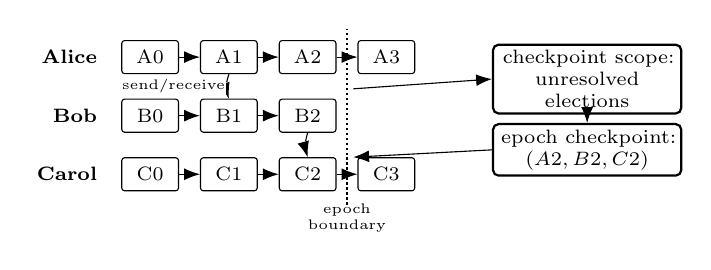
\begin{tikzpicture}[
  x=1cm,y=0.62cm,
  block/.style={draw,rounded corners=1pt,minimum width=.72cm,minimum height=.42cm,inner sep=1pt,font=\scriptsize},
  close/.style={draw,thick,rounded corners=2pt,text width=2.25cm,minimum height=.58cm,align=center,inner sep=2pt,font=\scriptsize},
  arr/.style={-{Latex[length=2mm]},thin},
  dep/.style={-{Latex[length=2mm]},dashed,thin}
]
\node[anchor=east,font=\scriptsize\bfseries] at (.45,3.2) {Alice};
\node[anchor=east,font=\scriptsize\bfseries] at (.45,2.0) {Bob};
\node[anchor=east,font=\scriptsize\bfseries] at (.45,.8) {Carol};
\node[block] (a0) at (1,3.2) {A0};
\node[block] (a1) at (2,3.2) {A1};
\node[block] (a2) at (3,3.2) {A2};
\node[block] (a3) at (4,3.2) {A3};
\node[block] (b0) at (1,2.0) {B0};
\node[block] (b1) at (2,2.0) {B1};
\node[block] (b2) at (3,2.0) {B2};
\node[block] (c0) at (1,.8) {C0};
\node[block] (c1) at (2,.8) {C1};
\node[block] (c2) at (3,.8) {C2};
\node[block] (c3) at (4,.8) {C3};
\draw[arr] (a0)--(a1); \draw[arr] (a1)--(a2); \draw[arr] (a2)--(a3);
\draw[arr] (b0)--(b1); \draw[arr] (b1)--(b2);
\draw[arr] (c0)--(c1); \draw[arr] (c1)--(c2); \draw[arr] (c2)--(c3);
\draw[dep] (a1.south) to[bend right=18]
  node[midway,left,fill=white,inner sep=.5pt,font=\tiny]{send/receive} (b1.north);
\draw[dep] (b2.south) to[bend right=16] (c2.north);
\draw[densely dotted,thick] (3.5,.18)--(3.5,3.78);
\node[font=\tiny,align=center] at (3.5,-.10) {epoch\\boundary};
\node[close] (cut) at (6.55,2.75) {checkpoint scope:\\unresolved elections};
\node[close] (rec) at (6.55,1.30) {epoch checkpoint:\\$(A2,B2,C2)$};
\draw[arr] (cut)--(rec);
\draw[arr] (3.58,2.55) -- (cut.west);
\draw[arr] (rec.west) -- (3.58,1.15);
\end{tikzpicture}
\caption{\sys keeps owner-authorized account chains independent.  Receive edges impose causality without a global log.  Epoch closure elects a safe set of unresolved slot elections and then a checkpoint frontier containing one finalized head per account.  The figure should remain in the final paper; replace labels with the implementation's exact object names if they differ.}
\Description{Three independent account chains with cross-account receive dependencies converge into a two-step epoch close consisting of a checkpoint scope and a epoch checkpoint.}
\label{fig:lattice}
\end{figure}

A transfer has two explicit steps.  A send reduces the source balance and creates a uniquely identified pending output.  A receive consumes that output after the source block is finalized.  This choice makes replay deterministic and prevents a recipient from crediting value that might later disappear.  It also means cross-account latency includes the source slot's finality plus the recipient's next block; Section~\ref{sec:limits} discusses this trade-off.

\subsection{Why broadcast alone is insufficient}

A reliable-broadcast payment system can guarantee that correct replicas never execute two different operations for the same sender sequence number.  If the sender equivocates, however, termination may be lost: different correct replicas can become locked on incompatible values.  For a one-shot payment this can be attributed to the faulty sender.  In a production ledger, the unresolved evidence must eventually be either retained as final history or discarded with a proof strong enough to permit a safe retry.

Dynamic stake adds a second problem.  Suppose validators change from epoch $e$ to $e+1$ while an old slot is only partially notarized.  The new committee must know whether voting for a conflicting retry would violate an old quorum intersection argument.  A single checkpoint hash is not enough unless it determines which old slots were finalized and which obligations were released.  Finally, new replicas need a bounded object from which they can authenticate the current balances, delegations, pending outputs, and account heads.

\sys resolves all three problems with a epoch checkpoint.  The record is not a block containing transactions.  It is the hash of a canonical map $\frontier_e:a\mapsto b$, where $b$ is the finalized head of account $a$ through epoch $e$, chained to the preceding checkpoint digest:
\begin{equation}
  \closehash_e = \hash(\textsf{RAI/CloseRecord}\parallel e\parallel
  \closehash_{e-1}\parallel\canon(\frontier_e)).
  \label{eq:closehash}
\end{equation}
Because each block commits to its parent, $\frontier_e$ transitively commits to all finalized account history.  Deterministic replay reconstructs balances, representatives, pending outputs, and consumed sends.  The close also supplies a certified release decision for every epoch-$e$ slot election omitted from the selected chains.

\subsection{Goals and non-goals}

\sys targets a permissioned or proof-of-stake validator set with weighted Byzantine faults and authenticated gossip.  It provides account ownership, transfer conservation, per-slot finality, checkpointed reconfiguration, and safe retry.  It is \emph{not} a general state-machine-replication protocol.  An operation that requires mutually distrusting writers to update one shared object still needs a different abstraction, such as consensus, a shared-account protocol, or an application-specific escrow construction.  This specialization is central: \sys gains concurrency by exposing the ownership structure instead of hiding it behind one ordered log.

\section{Model and Ledger Semantics}
\label{sec:model}

\paragraphhead{Participants and network.}
Validators communicate over authenticated reliable channels.  Safety holds in asynchrony; liveness assumes a period of partial synchrony and eventual delivery among correct online validators.  Owners may be Byzantine and may sign conflicting blocks.  For each frozen committee $Q$, let $W_Q$ be total stake, at most $F_Q$ be Byzantine stake, and $P_Q\ge F_Q$ be an optimistic slack parameter.  We require
\begin{equation}
    W_Q > 3F_Q + 2P_Q.
    \label{eq:weightassumption}
\end{equation}
The common $W=3F+2P+1$ cardinality form appears in fast-path BFT protocols; \sys applies the inequalities to exact stake weight.

\paragraphhead{Account blocks.}
An account slot is $(a,s)$, with $s\ge1$.  A block body contains
\[
 (a,s,\mathsf{parent},\mathsf{sends},\mathsf{receives},\mathsf{representative}),
\]
and an owner signature over a domain-separated canonical encoding.  A send entry $(d,x)$ has a unique reference $(\hash(B),i)$, and a receive lists such references.  Validity requires a correct owner signature, the expected parent and sequence, nonnegative replayed balance after sends, no duplicate receive, and a finalized source block for every receive.

\paragraphhead{Derived state.}
Replaying finalized chains yields
\[
  \ledger=(\mathsf{bal},\mathsf{rep},\mathsf{pending},\mathsf{received}).
\]
Here \(\mathsf{bal}\) and \(\mathsf{rep}\) abbreviate the balance and representative maps. This tuple is derived, not separately voted upon.  Genesis fixes initial balances and owner keys.  A send moves value from a balance into the pending-output set; a receive moves the same value from pending to the destination balance.  Thus the total of spendable balances plus pending outputs is invariant.

\paragraphhead{Election identifiers.}
The protocol runs three logical election types:
\[
 \Slot(a,s,e), \qquad \Cut(e,r), \qquad \Record(e,r),
\]
where $e$ is an epoch and $r$ is a close retry round.  The pair $(a,s)$ denotes the persistent account slot, while $\Slot(a,s,e)$ denotes its epoch-scoped slot election.  Slot-election values are block hashes.  Close values are hashes of locally retained canonical payloads (their hash preimages).  Only blocks, signed reports, and signed votes are durable authenticated wire objects.  Certificates, conflicts, outcomes, frontiers, and committees are deterministic facts derived from those objects.

\paragraphhead{Lagged committees.}
Delegated stake in an installed checkpoint state derives the committee for that epoch.  An election in epoch $e$ is checked against the two available lagged snapshots $Q_{e-3}$ and $Q_{e-2}$ (with genesis substitutions for early epochs).  A vote is logically scoped to each committee, even when one wire signature compresses identical actions for overlapping membership.  The $e-2$ installed checkpoint state also supplies the governing finalized account frontier.  This arrangement allows at most one open and one closing epoch while avoiding a committee that depends on the result it is currently certifying.

\paragraphhead{Required properties.}
For every execution satisfying the stake bound, \sys must ensure: (1) only an owner-authorized block can debit an account; (2) no two different blocks finalize for one account slot; (3) a correct validator never supports a conflicting retry until a certified close releases its earlier obligation; (4) epoch checkpoints form one hash chain and preserve every previously finalized prefix; and (5) every correct owner's admissible operation and every started close eventually settles during synchrony.  The formal statement distinguishes operation liveness from Byzantine-owner liveness: an equivocating owner may wait until epoch close before retrying.

\section{One Weighted Election Kernel}
\label{sec:kernel}

Every election/committee pair uses the same three vote kinds.  A validator emits at most one \emph{first} vote.  A first vote also counts as a notarization vote.  After seeing first-vote weight strictly greater than $F_Q+P_Q$ for value $x$, a validator may send a second-look notarization vote for $x$.  It sends a final vote only when all committee-local support it has issued is compatible with $x$; afterward it is locked.  A timeout notarization vote becomes valid when
\begin{equation}
 \mathsf{allVotes}(Q,I)-\mathsf{maxVotes}(Q,I)>F_Q+P_Q.
 \label{eq:timeout}
\end{equation}
This monotone predicate proves that too much weight lies outside every candidate for a fast decision.

\begin{table}[t]
\caption{Committee-local certificate thresholds.  A certificate is a local collection of individually authenticated votes, not a separate wire object.}
\label{tab:thresholds}
\centering
\small
\begin{tabularx}{\columnwidth}{@{}lXl@{}}
\toprule
Kind & Required signer weight in $Q$ & Restriction \\
\midrule
Notarization & $W_Q-F_Q-P_Q$ notarization votes & any value \\
Fast & $W_Q-P_Q$ first votes & non-timeout \\
Final & $W_Q-F_Q-P_Q$ final votes & non-timeout \\
Timeout & $W_Q-F_Q-P_Q$ timeout notarization votes & Eq.~\eqref{eq:timeout} \\
\bottomrule
\end{tabularx}
\end{table}

The local result is one of $\mathsf{notarized}(x)$, $\mathsf{fast}(x)$, $\mathsf{final}(x)$, or timeout.  Results from the two lagged committees merge deterministically.  Global fast/final status requires compatible support for the same $x$ in both committees.  A timeout in either committee, or terminal certificates for different values, yields non-final conflict evidence.  Overlap between the committees is harmless because vote histories and locks are interpreted per $(I,Q)$.

\begin{algorithm}[t]
\caption{Committee-local action at validator $v$ for election $I$}
\label{alg:kernel}
\small
\begin{algorithmic}[1]
\State first-vote the locally admissible value $x$ once
\If{first-vote weight$(x)>F_Q+P_Q$ and $x$ is admissible}
  \State notarize $x$ (second look)
\EndIf
\If{Eq.~\eqref{eq:timeout} holds}
  \State notarize $\timeout$
\EndIf
\If{notarization$(x)\ge W_Q-F_Q-P_Q$ and all prior support is in $\{x\}$}
  \State final-vote $x$ and lock this $(I,Q)$ instance
\EndIf
\State derive fast/final/timeout certificates from the vote store
\end{algorithmic}
\end{algorithm}

The threshold intersections give the key incompatibility property.  A fast certificate for $x$ leaves at most $F_Q+P_Q$ signer weight outside $x$, so no other value can pass the strict second-look threshold and timeout cannot become valid.  A final certificate and a different notarization certificate intersect in weight
\[
 2(W_Q-F_Q-P_Q)-W_Q = W_Q-2F_Q-2P_Q > F_Q,
\]
which contains correct stake and contradicts the support lock.  Consequently, no value different from a locally fast/final $x$ can obtain notarization, and two global finalized values are impossible.  The kernel adapts the counting structure of Kudzu~\cite{shoup2025kudzu}; proposal dissemination, account admissibility, multi-committee composition, and close carry are specific to \sys.

\section{Account Slots}
\label{sec:slots}

\subsection{Admissibility and stable prefixes}

A validator accepts a block only after verifying its owner signature and canonical body.  It votes only if the parent block is complete and every strict non-genesis ancestor is already finalized.  We call this the \emph{stable-prefix} rule.  It is stronger than merely knowing the ancestor or seeing it notarized: an unresolved or later-released block cannot become the foundation of a descendant that finalizes in another epoch.

For epoch $e\ge2$, the block must also descend from the account frontier certified in installed checkpoint state $e-2$.  During an epoch-$e$ close drain, admissibility is evaluated against a frozen close input: every post-$e-1$ ancestor must be the selected block of an election in the decided cut, and receive dependencies must resolve in the close-local replay.  Thus an epoch-$e$ close cannot accidentally incorporate a concurrently finalized epoch-$(e+1)$ block.

A validator records every non-timeout vote as an obligation for that slot election.  It may vote for a conflicting block in a later election for the same $(a,s)$ only if a certified installed checkpoint state has either excluded the old election or installed a ledger that omits that old block.  Local timeouts and local garbage collection are not release evidence.

\subsection{Fast finality and unresolved notarization}

\begin{figure}[t]
\centering
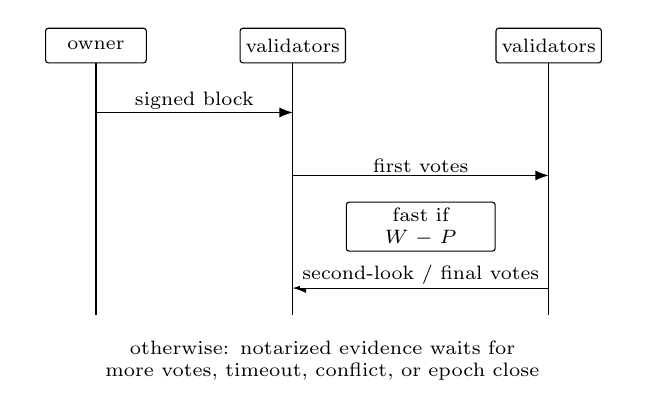
\begin{tikzpicture}[x=1cm,y=1cm,font=\scriptsize,
  msg/.style={-{Latex[length=1.7mm]},thin},
  participant/.style={draw,rounded corners=1pt,minimum width=1.28cm,minimum height=.44cm,inner sep=2pt,align=center},
  result/.style={draw,rounded corners=1pt,text width=1.75cm,minimum height=.58cm,inner sep=2pt,align=center}]
\node[participant] (o) at (.75,4.20) {owner};
\node[participant] (v1) at (3.25,4.20) {validators};
\node[participant] (v2) at (6.50,4.20) {validators};
\draw[thin] (o.south) -- (.75,.78);
\draw[thin] (v1.south) -- (3.25,.78);
\draw[thin] (v2.south) -- (6.50,.78);
\draw[msg] (.75,3.35) -- node[above,fill=white,inner sep=1pt]{signed block} (3.25,3.35);
\draw[msg] (3.25,2.55) -- node[above,fill=white,inner sep=1pt]{first votes} (6.50,2.55);
\node[result] at (4.875,1.90) {fast if\\$W-P$};
\draw[msg] (6.50,1.12) -- node[above,fill=white,inner sep=1pt]{second-look / final votes} (3.25,1.12);
\node[align=center,text width=7.25cm] at (3.625,.20)
  {otherwise: notarized evidence waits for\\more votes, timeout, conflict, or epoch close};
\end{tikzpicture}
\caption{Slot path.  A fast certificate finalizes directly.  A notarization alone completes the election evidence but does not finalize the account slot; epoch close either includes the block on the certified chain or releases the election's obligation.}
\Description{A message sequence chart showing client submission, validator first votes, optional fast finalization, final votes, timeout evidence, and settlement by epoch closure.}
\label{fig:slotpath}
\end{figure}

If both committees derive a compatible fast or final certificate, the block immediately finalizes and replay advances the account.  This is the normal path.  Notarization alone has a deliberately weaker meaning: enough evidence exists that the block cannot be forgotten when closing the epoch, but the slot is not yet safe to expose as final.  The election may subsequently final-vote the same block, time out, or reveal incompatible terminal evidence.  This separation avoids treating a partially propagated notarization as permanent ledger state while ensuring it is captured by the checkpoint scope.

A timeout never creates an empty block and never skips an account sequence number.  It only settles the epoch-scoped slot election; the persistent account slot $(a,s)$ remains unfilled.  The epoch checkpoint determines whether the owner may retry the same account slot in a later epoch.  Because descendants require finalized ancestors, later account progress cannot route around a timed-out slot election until the close has selected its block or certified release of its obligation.

\section{Closing an Epoch without Ordering Transactions}
\label{sec:close}

\sys starts closing epoch $e$ only after epoch $e-1$ is closed.  It immediately opens $e+1$, so ordinary work continues while $e$ closes.  The closing protocol has two logical elections, each with retry rounds and a carry rule.

\subsection{Step 1: certify a safe checkpoint scope}

At close start, every validator signs a report containing (i) pending epoch-$e$ slots it has observed and (ii) every unreleased non-timeout vote obligation it has created.  A report equivocator is excluded from fresh report-derived visibility.  Vote-derived visibility is monotone: any slot with valid-vote weight greater than Byzantine weight remains visible even if reports arrive late.

A candidate cut $C_e$ is the canonical set of visible $\Slot(a,s,e)$ identifiers.  Before voting for
\[
 h_C=\hash(\textsf{RAI/CloseCut}\parallel e\parallel\canon(C_e)),
\]
a validator must possess a joint report proof of weight at least $W_Q-F_Q$ in every close committee and include every slot election visible in those reports.  It also validates a start witness for every cut entry.  Only $h_C$ is voted; $C_e$ remains a retained, hash-indexed payload.

Why does the cut contain every safety obligation?  Any slot certificate capable of finishing has weight at least $W_Q-F_Q-P_Q$.  Intersecting it with a report quorum of weight $W_Q-F_Q$ yields
\[
 W_Q-2F_Q-P_Q > F_Q+P_Q.
\]
After removing Byzantine stake, enough correct reporters remain to expose the slot.  Thus a decided cut may safely exclude late noise, but cannot omit a pre-close quorum that could still affect safety.

After a cut decision, validators reconstruct its payload, freeze
$(\closehash_{e-1},\frontier_{e-1},C_e)$ as the close input, and resume every included unfinished slot.  Slots outside the cut are not resumed and will be released by the close.  Included slots drain to fast/final, notarized, timeout, or certified conflict evidence.

\subsection{Step 2: certify a checkpoint frontier}

Once the cut is drained, each validator replays only cut elections from the previous certified frontiers.  The deterministic resolver obeys three principles: a globally fast/final block and its stable ancestors must be included; timeout or known conflict omits the slot election; and a single non-conflicting notarized candidate may be included if it produces a valid account chain.  There is no arbitrary tie-breaker when conflict is known.

The resulting canonical map $\frontier_e$ contains one head per account.  Validators vote for the checkpoint digest in Eq.~\eqref{eq:closehash}.  A decided epoch checkpoint has four effects, in normative order:
\begin{enumerate}[leftmargin=1.3em,itemsep=1pt,topsep=2pt]
\item finalize every block on each selected chain that was not already final;
\item mark the obligations of every other epoch-$e$ slot election as certifiedly released;
\item replay the selected chains to install balances, pending outputs, receives, and representatives; and
\item derive the next exact-proportional stake committee from installed balances and delegation.
\end{enumerate}
The cut supports this derivation but is not an extra field in the durable checkpoint hash.  A bootstrapper obtains a epoch checkpoint, reconstructs its checkpoint frontier, verifies the parent-linked account chains and close-hash chain, and replays state.

\subsection{Retry rounds, carry, and reconciliation}

A close round may decide, converge on a notarized hash, or die.  A notarized non-timeout hash becomes a \emph{mandatory carryover}; the next round must first-vote that same hash unless positive certificate-level carryover-invalidation proof exists.  Death is either a timeout certificate or incompatible terminal certificates proving that no common fast/final value can emerge.  A local clock expiry or changed fresh preference is insufficient.  Once all correct validators carry the same admissible hash, their weight alone reaches the fast threshold.

Close values can be large even though close votes are constant-size.  Each voter retains the canonical payload it validated.  A lagging replica asks for a delta from a locally known base hash to the target hash.  It applies additions/removals, recomputes the target hash, and revalidates every element against its block/report/vote store.  Deltas are availability hints, not authority: a malformed or incomplete delta cannot create a valid close vote or certificate.  The prototype must quantify the effectiveness and worst-case amplification of this mechanism (Section~\ref{sec:eval}).


\section{Protocol Lifecycle and Adversarial Cases}
\label{sec:lifecycle}

This section makes the state transitions explicit and explains why several apparently simpler alternatives are unsafe.  It is also a blueprint for the implementation's event loop and test oracle.

\subsection{Epoch state machine}

A correct validator stores an epoch in one of three states: open, closing, or closed.  At most two adjacent epochs are active.  While $e$ is open, its slot elections accept new account blocks.  Closing may start only when $e-1$ is already closed.  The transition to closing freezes no transactions by itself: the validator emits its report, starts the close-cut instance, and immediately opens $e+1$.  Slot elections in $e$ remain enabled only if the decided cut later includes them; slots in $e+1$ proceed against the older certified frontier enforced by the stable-prefix rule.

\begin{table}[t]
\caption{Normative epoch transitions and durable effects.  ``Durable'' means the state survives crash recovery and cannot be reconstructed from a local timer alone.}
\label{tab:lifecycle}
\centering
\small
\begin{tabularx}{\columnwidth}{@{}lXX@{}}
\toprule
Phase & Enabled work & Durable transition \\
\midrule
Open $e$ & accept/validate blocks; run $\Slot(\cdot,\cdot,e)$ & fast/final slot certificates \\
Start close & sign report; start $\Cut(e,0)$; open $e+1$ & report object and vote obligations \\
Cut decided & reconstruct $C_e$; resume only $q\in C_e$ & decided cut hash and payload \\
Drain & finish every $q\in C_e$ & slot votes, timeouts, conflicts \\
Record decided & reconstruct $\frontier_e$; replay and install & $\closehash_e$, frontiers, final/release state \\
Closed $e$ & prune volatile caches; derive committee & installed close and committee \\
\bottomrule
\end{tabularx}
\end{table}

\begin{algorithm}[t]
\caption{Condensed close controller at validator $v$}
\label{alg:close}
\small
\begin{algorithmic}[1]
\Procedure{StartClosing}{$e$}
  \Require $e$ open and $e-1$ closed
  \State persist and gossip signed report $R_v[e]$
  \State open epoch $e+1$; start $\Cut(e,0)$
\EndProcedure
\Statex \textbf{upon decision $\Cut(e,r)=h_C$ do}
  \State $C_e\gets\Call{ObtainAndValidate}{h_C}$; persist $C_e$
  \ForAll{$q\in C_e$ not terminal} \State resume $q$ with a running timer \EndFor
\Statex \textbf{upon all $q\in C_e$ terminal do}
  \State $\frontier\gets\Call{ResolveAndReplay}{\frontier_{e-1},C_e}$
  \State retain $\frontier$ by hash; start/continue $\Record(e,\cdot)$
\Statex \textbf{upon decision $\Record(e,r)=h_F$ do}
  \State $\frontier_e\gets\Call{ObtainAndValidate}{h_F}$
  \State finalize selected chains; release all other epoch-$e$ slots
  \State replay ledger, derive committee, persist closed state
\end{algorithmic}
\end{algorithm}

Every transition in Algorithm~\ref{alg:close} is idempotent.  A crash after persisting a decision but before applying its effects repeats validation and replay.  A crash before the decision loses no authority because the signed votes remain in the object store.  The implementation should enforce the normative order on record installation: first verify the checkpoint digest and parent close, then materialize the frontier, then finalize selected blocks/release omitted slot-election obligations, then replay balances and delegation, and only then enable committee-dependent work.

\subsection{An equivocation walkthrough}

Assume Alice's certified frontier before epoch $e$ is block $A_4$, and Alice signs two blocks $A_5$ and $A'_5$ for the same slot.  Validators in one network region first-vote $A_5$ while others first-vote $A'_5$.  Three outcomes illustrate the design.

\paragraphhead{One block fast-finalizes.}
If $A_5$ reaches the fast threshold in both committees, certificate incompatibility prevents $A'_5$ from being notarized.  $A_5$ finalizes immediately.  Reports still mention any unreleased vote obligations, but the close replay has only one valid finalized continuation and commits a frontier at or after $A_5$.

\paragraphhead{The split is terminal.}
If incompatible terminal certificates appear, the slot election's merged result is conflict/timeout.  Report quorum intersection forces the slot election into $C_e$.  The drain records the positive conflict evidence, the resolver keeps Alice's frontier at $A_4$, and the installed checkpoint state releases the vote obligations for both candidates.  Alice may then submit a new block for slot 5 in a later permitted epoch; validators reject such a retry before the close because their old votes are still active.

\paragraphhead{Only one notarization is known.}
If $A_5$ is notarized but not final and no conflict is known, the cut includes the slot election and the close-local resolver may select $A_5$, provided its parent and receive dependencies are valid.  The epoch checkpoint then finalizes it.  If later-gossiped evidence reveals a conflict \emph{after} the close decision, it cannot rewrite history: the decided, hash-checked historical frontier is authoritative.  Conversely, if the conflicting evidence arrives before a fresh close-record vote, the fresh resolver omits the slot election.  This distinction is why historical admissibility is monotone after certificate support while fresh preference remains evidence-sensitive.

A block or vote first learned after the cut decision but not represented in $C_e$ cannot create an epoch-$e$ slot-election obligation.  It is retained for audit, but the close exclusion releases it.  This rule bounds closing despite asynchronous gossip; the report-intersection proof ensures it cannot discard a quorum that was already capable of finishing before close.

\subsection{Why the design has two close elections}

A tempting design is to vote directly on a checkpoint frontier at close start.  It fails because validators may construct maps from different unresolved universes.  One validator might omit a notarized slot it has not yet learned, while another has already voted in that slot and must preserve the obligation.  Requiring the frontier vote to wait for ``all evidence'' is not implementable in an asynchronous network.  The cut election first agrees on a finite evidence domain with a quorum-intersection argument; only then can deterministic replay produce a stable close-record candidate.

Another alternative is to include the entire cut and frontier in every vote.  This simplifies retrieval but turns validator signatures and vote gossip into $O(U_e+A_e)$ messages.  Hash-only voting isolates consensus evidence from data movement.  Its price is explicit payload retention and reconciliation, which must be measured and protected against resource-exhaustion attacks.

\subsection{Attack-oriented design rationale}

\begin{table*}[t]
\caption{Representative adversarial cases and the protocol mechanism that must be exercised in tests.}
\label{tab:attacks}
\centering
\small
\begin{tabularx}{\textwidth}{@{}p{.16\textwidth}p{.24\textwidth}X X@{}}
\toprule
Adversarial action & Risk in a simpler design & \sys defense & Required implementation test \\
\midrule
Owner signs two blocks for one slot & double spend or indefinite lock & one-first-vote/committee locks; conflict evidence; close-record release & deterministic split-vote schedule, crash, close, then retry \\
Late votes appear during close & omitted quorum later finalizes & report/certificate intersection forces every pre-close safety obligation into the cut & delay just enough votes until before/after cut decision \\
Reporter equivocates & two validators construct incompatible visibility sets & signed report store detects signer equivocation; fresh report visibility excludes it; vote visibility remains monotone & send two reports to disjoint peers and verify convergent cut behavior \\
Close candidate splits & successive rounds abandon a value that could still decide & notarized mandatory carryover is mandatory until timeout/conflicting terminal evidence proves death & delay payload to some validators; verify no timeout-first vote while reconstructing \\
Peer sends malicious delta & corrupt frontier or unbounded allocation & chunk/resource limits; recompute target hash; validate every element from authenticated atoms & fuzz edits, duplicate keys, oversized chunks, wrong base/target hashes \\
Old and new committees overlap & one signature counted inconsistently or cross-epoch retry violates old lock & logical vote scope per $(I,Q)$; two lagged snapshots; certified $e-2$ release/frontier guards & random weighted overlaps and committee-change model checking \\
Replica restarts mid-install & committee derived from partially applied state & write-ahead decision record and idempotent normative replay order & crash after every persistence point and compare recovered state root \\
\bottomrule
\end{tabularx}
\end{table*}

\paragraphhead{Notarization is not finality.}
Treating notarization as final would shorten the slow path, but it would force every close and retry rule to preserve a value that has not passed the final-vote support lock.  \sys instead uses notarization as evidence that the candidate must be resolved.  This gives the close freedom to include a unique valid candidate or omit a known conflict without violating a client-visible finality promise.

\paragraphhead{Carry waits for data.}
A validator that sees a live carried hash but lacks its payload must retrieve the payload; it must not first-vote timeout merely because retrieval is slow.  Otherwise the successor round could manufacture conflicting terminal evidence against a value whose previous-round quorum is still capable of leading to a decision.  Transport backpressure therefore cannot be allowed to masquerade as consensus evidence.

\paragraphhead{Two lagged snapshots.}
Using only the newest committee would let a close whose result determines stake also determine the voters authorized to certify that result.  Using only one older committee creates a sharp handoff: evidence accepted by the old committee can race with retries voted by the new.  Requiring compatible results from two certified lagged snapshots retains an intersection of governed history across the overlap.  The cost is duplicate logical vote accounting and a stronger assumption: the Byzantine-weight bound must hold in both snapshots.

\paragraphhead{No certificate wire objects.}
A certificate is a deterministic predicate over immutable votes.  Accepting separately signed or aggregated certificate messages as authority would introduce a fourth consensus object class, arrival-order ambiguities, and recovery state that could disagree with the underlying vote set.  Implementations may cache signer bitmaps or aggregate signatures as accelerators, but recovery and correctness checks must be able to derive the same result from authenticated votes.

\section{Correctness and Cost}
\label{sec:correctness}

The supplementary material gives state-machine pseudocode and full proofs~\cite{raiSupplement}.  We summarize the proof structure and the costs that matter to an implementation.

\paragraphhead{Slot safety.}
For one committee, the threshold-intersection argument in Section~\ref{sec:kernel} prevents a different value from being notarized after a fast/final value.  The deterministic cross-committee merge finalizes only one common value.  The persistent per-slot map rejects a second finalization from any later epoch.  The stable-prefix rule then extends uniqueness from one slot to the account chain: a correct validator cannot help a descendant finalize over an unresolved or released ancestor.

\paragraphhead{Safe retry across epochs.}
Every correct non-timeout vote remains an obligation for its slot election until the installed close either selects that block on the certified account chain or omits the election with release evidence.  Report-quorum intersection forces every potentially finishing pre-close slot election into the cut.  Therefore a later conflicting retry can gather a quorum only after the old obligation is certifiedly released.  Lagged installed checkpoint state ensures that voters separated by committee changes apply the same governing frontier and release decision.

\paragraphhead{Checkpoint safety.}
The close-cut election chooses at most one hash. Historical validation preserves its hash-checked payload after certificate support. The close-record election likewise chooses at most one hash. Equation~\eqref{eq:closehash} chains that decision to the preceding close, while frontier replay requires all prior finalized blocks. Hence correct replicas install one cumulative checkpoint sequence and derive the same stake state.

\paragraphhead{Liveness.}
During synchrony, a popular first-vote value receives second-look votes; otherwise Eq.~\eqref{eq:timeout} eventually enables a timeout certificate.  Thus an unlocked close round decides, creates a mandatory carryover, or obtains carryover-invalidation proof.  A carry is reconstructed and fast-decided in the next round; death unlocks fresh canonical construction.  Under finite evidence and deterministic replay, fresh preferences eventually converge.  The decided cut contains a finite set of started slot elections, each of which drains, after which the epoch checkpoint decides and the next committee is installed.

\begin{table}[t]
\caption{Analytical cost before implementation optimizations.  $n$ is committee size, $A_e$ the number of accounts whose frontier changes in epoch $e$, and $U_e$ the number of unresolved slot elections in the cut.  Point-to-point transmissions depend on the gossip overlay.}
\label{tab:cost}
\centering
\small
\begin{tabularx}{\columnwidth}{@{}lXX@{}}
\toprule
Operation & Authenticated objects & Retained/derived state \\
\midrule
Fast slot & one block, $O(n)$ votes per committee & block plus $O(n)$ vote records \\
Slow slot & one block, up to $O(n)$ first/notar/final votes & same, until close/GC \\
Checkpoint scope & $O(n)$ reports, $O(n)$ votes per round & $O(U_e)$ cut payload \\
Epoch checkpoint & $O(n)$ votes per round & $O(A_e)$ sparse frontier delta; full map logically $O(A)$ \\
Bootstrap & checkpoint plus account-chain data & replay state proportional to retained history/checkpoint scheme \\
\bottomrule
\end{tabularx}
\end{table}

The base protocol uses individual signatures so any replica can derive a certificate from its vote store.  Naive all-to-all delivery is $O(n^2)$ point-to-point messages per vote phase, although each logical phase contains only $O(n)$ distinct signed vote objects.  The evaluation must separate object bytes from duplicate transport bytes and show whether inventory gossip, batching, and aggregate verification make this acceptable at the intended committee size.

\section{Implementation Plan and Reserved Description}
\label{sec:impl}

This section is intentionally written as a concrete fill-in plan rather than a fictional implementation report.  The final paper should describe a single reproducible prototype and use the same code path for normal slots, closing, recovery, and experiments.

\subsection{Architecture to implement}

\begin{figure}[t]
\centering
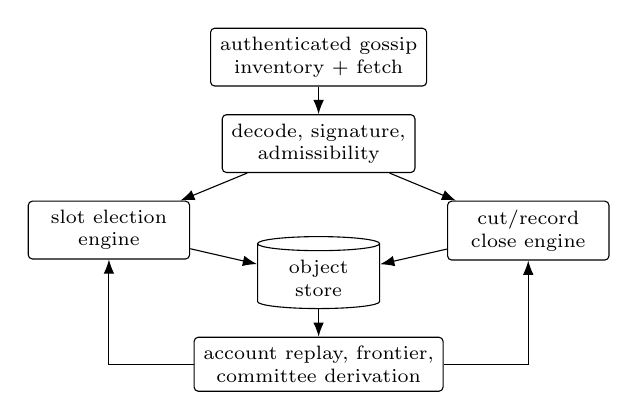
\begin{tikzpicture}[font=\scriptsize,node distance=3.5mm and 4mm,
  comp/.style={draw,rounded corners=1.5pt,minimum height=.50cm,minimum width=2.05cm,align=center},
  store/.style={draw,cylinder,shape border rotate=90,aspect=.18,minimum height=.67cm,minimum width=1.55cm,align=center},
  arr/.style={-{Latex[length=1.8mm]},thin}]
\node[comp] (net) {authenticated gossip\\inventory + fetch};
\node[comp,below=of net] (val) {decode, signature,\\admissibility};
\node[comp,below left=of val] (slot) {slot election\\engine};
\node[comp,below right=of val] (close) {cut/record\\close engine};
\node[store,below=8mm of val] (objects) {object\\store};
\node[comp,below=of objects] (replay) {account replay, frontier,\\committee derivation};
\draw[arr] (net)--(val); \draw[arr] (val)--(slot); \draw[arr] (val)--(close);
\draw[arr] (slot)--(objects); \draw[arr] (close)--(objects); \draw[arr] (objects)--(replay);
\draw[arr] (replay.west) -| (slot.south); \draw[arr] (replay.east) -| (close.south);
\end{tikzpicture}
\caption{Target validator architecture.  The final implementation section should map each box to modules/threads and identify every persistent boundary.  Keep validation before indexing, and make both election engines derive certificates from the same immutable object store.}
\Description{Validator architecture with authenticated gossip and validation feeding slot and close election engines, an immutable object store, and deterministic account replay and committee derivation.}
\label{fig:implementation}
\end{figure}

\paragraphhead{Runtime and networking.}
Implement the validator in \ImplLanguage.  Report the exact asynchronous runtime, serialization version, and commit identifier \EvalCommit.  Use an authenticated transport \ImplTransport with one stream/class for blocks and one for small control objects, explicit bounded queues, duplicate suppression by object hash, and peer inventory summaries.  The paper must state whether broadcast is eager all-to-all, overlay gossip, or hybrid; how retries and backpressure work; and whether experiments include TLS/QUIC handshakes or pre-established sessions.

\paragraphhead{Cryptography and canonical encoding.}
Use \ImplCrypto.  Every signature must bind protocol version, object kind, election id, committee id, and value.  Define one canonical byte encoding and include round-trip/fuzz tests that reject alternate encodings.  Certificates should be represented as signer bitmaps plus references to immutable vote objects, not accepted as independently trusted messages.  Report individual verification, batch verification, and hash throughput; measure the percentage of CPU spent on each.

\paragraphhead{Storage and recovery.}
Use \ImplStorage. At minimum, persist blocks by hash; votes by election, committee, kind, value, and signer; reports by epoch and signer; account heads; close payloads; and installed checkpoint states.  The final text must identify which writes are synchronous before acknowledging a client, how incomplete batches recover, and which derived indexes can be rebuilt.  Crash recovery should replay the last installed close, then scan post-close objects to reconstruct election state without trusting cached certificates.

\paragraphhead{Execution and close reconstruction.}
Use a per-account scheduler so unrelated block validation/replay can run concurrently while preserving account sequence.  Represent a frontier version as a persistent sorted map or Merkleized sparse map; store deltas against the prior decided frontier and against every locally voted close candidate until the instance decides.  Implement delta fetch with chunking, hashes per chunk, resource limits, and fallback full-payload retrieval.  The paper should include the measured cache hit rate, median delta size, and worst-case reconstruction time.

\paragraphhead{Engineering optimizations.}
Evaluate, rather than assume, the benefit of: vote batching; batch signature verification; inventory compression; coalescing identical logical votes for overlapping committees; parallel account replay; and incremental checkpoint digesting.  State the final code size (\ImplLOC), test-suite size, and number of lines reused from third-party libraries.  Include a public or anonymized artifact only after checking it for author-identifying metadata.

\begin{table}[t]
\caption{Implementation details to replace before submission.  Do not leave generic product names without version, configuration, and persistence semantics.}
\label{tab:impl}
\centering
\small
\begin{tabularx}{\columnwidth}{@{}lX@{}}
\toprule
Item & Required final content \\
\midrule
Runtime & \ImplLanguage; worker topology and queue bounds \\
Transport & \ImplTransport; fanout, MTU, retry, congestion control \\
Crypto & \ImplCrypto; key sizes, batching, signer bitmap format \\
Storage & \ImplStorage; WAL/fsync policy and recovery algorithm \\
State map & concrete frontier data structure and delta encoding \\
Artifact & \EvalCommit; build command, dependency lockfile, license \\
\bottomrule
\end{tabularx}
\end{table}


\subsection{Validation, testing, and artifact structure}

A protocol implementation should not be validated only by end-to-end throughput runs.  The final artifact should contain a small deterministic reference model, a production validator, and a differential test harness.  The reference model may be single-threaded and inefficient, but it must implement the normative order of validation, certificate derivation, close resolution, and installation from the supplement.  After every generated event, the harness compares the production node's durable observations with the model: finalized-slot map, active vote obligations, decided checkpoint digests, reconstructed frontiers, replayed balances, and derived committees.  Derived caches may differ; authoritative state may not.

\paragraphhead{Schedule exploration.}
Build a deterministic in-process network that controls message delivery, duplication, disconnection, and restart.  Use seeded randomized schedules with 4--10 validators to explore overlapping committees, split first votes, report equivocation, late certificate completion, close carry, and payload delay.  Preserve every failing seed and minimize it to a regression test.  In addition to random testing, enumerate the small cases most likely to expose safety bugs: two candidate values, two committees with partial membership overlap, one Byzantine signer, and crashes at each durable transition in Table~\ref{tab:lifecycle}.

\paragraphhead{Property-based ledger tests.}
Generate valid and invalid account chains with sends, receives, representative updates, and retries.  Check authorization, sequence continuity, send uniqueness, receive-at-most-once, nonnegative balances, and global value conservation after every finalized block and close replay.  Generate malformed canonical encodings, duplicate map keys, integer boundaries, cycles, missing parents, receives from non-final sends, and blocks whose logical slot disagrees with the election id.  The validator must reject these inputs before indexing them by hash.

\paragraphhead{Crash consistency.}
Instrument the storage layer with failpoints after every write, WAL flush, batch commit, and state-machine callback.  Restart from the same database and require that the node either exposes the previous installed close or completes the same idempotent transition; it may never expose a committee derived from partially replayed state.  Run the same campaign during slot finality, cut decision, cut-payload reconstruction, close-record decision, and pruning.  Report the number of failpoints and the longest recovery path in the final paper.

\paragraphhead{Adversarial resource tests.}
Fuzz inventory messages, reconciliation deltas, signer bitmaps, and batches under strict per-peer budgets.  A Byzantine peer should be able to consume only configured bandwidth, memory, and verification work before being throttled.  In particular, delta application must check base hash, target hash, ordering, duplicate keys, chunk count, and maximum reconstructed size before allocating the complete map.  Measure rejection throughput as well as valid throughput so the evaluation does not assume well-formed traffic.

\placeholderfigure{2.0in}{
Four bars or line groups for the primitive operations that explain end-to-end cost: (1) individual and batch signature verification versus batch size; (2) object-store append/fsync and indexed lookup; (3) account-block validation/replay versus sends/receives per block; and (4) close-delta encode/apply/hash versus changed frontier entries. Report median and p99, CPU model, library versions, and whether data is hot or cold.}{Implementation microbenchmarks.  Replace with measured primitive costs and use the results to explain the bottleneck observed in the end-to-end evaluation.}

\paragraphhead{Artifact layout.}
Package the exact source revision, dependency lockfiles, build container, deployment manifests, workload generator, fault-injection scripts, plotting code, raw per-run measurements, and seeds for every published graph.  A one-command local smoke test should execute a small transfer, an equivocation, an epoch close, a certified release, and restart recovery.  The anonymized submission artifact must remove repository owners, cloud account identifiers, image registries, and embedded author paths while retaining license and provenance for third-party code.

\section{Evaluation Plan and Reserved Results}
\label{sec:eval}

The evaluation should answer five questions: (RQ1) how much throughput and latency does account-parallel finality provide? (RQ2) what overhead does the two-committee election kernel add? (RQ3) how expensive is epoch closure as unresolved slot elections and account count grow? (RQ4) how quickly does certified release recover from owner equivocation and replica faults? (RQ5) which CPU, network, and storage resources limit scaling?

\subsection{Methodology}

\paragraphhead{Testbeds.}
Use both a controlled LAN and a geo-distributed WAN.  Report \ImplMachine and \ImplRegions, operating-system/kernel versions, NIC limits, clock synchronization, placement, and whether client machines are separate.  Run committees of 4, 10, 25, 50, and 100 validators where feasible.  Repeat each data point for at least five independent runs after warm-up; plot medians with dispersion and include raw per-run data in the artifact.

\paragraphhead{Baselines.}
\begin{sloppypar}
Use three baseline classes. First, select HotStuff~\cite{yin2019hotstuff}, Tendermint~\cite{buchman2019tendermint}, or Simplex~\cite{chan2023simplex} as the low-latency leader-based BFT baseline. Second, select Bullshark~\cite{spiegelman2022bullshark}, Mysticeti-C~\cite{babel2025mysticeti}, or Shoal\allowbreak{}++~\cite{arun2025shoalpp} as the high-throughput DAG baseline. Third, implement a broadcast-only payment baseline modeled on FastPay~\cite{baudet2020fastpay} or Astro~\cite{collins2020astro}.  Use the same transaction encoding, signatures, batch size, transport, validator placement, and durability setting whenever possible.  If code reuse prevents a controlled comparison, state the incompatibility and present both a same-framework microbenchmark and an end-to-end published-system comparison without conflating them.
\end{sloppypar}

\paragraphhead{Workloads.}
Generate (1) independent-account transfers; (2) Zipf-distributed hot accounts; (3) send/receive chains of depth 1--32; (4) many recipients crediting concurrently; (5) owner equivocations at 0.01--10\%; and (6) stake/delegation churn at close.  Vary block payload from 256~B to 16~KiB, epoch duration, account population, and the number $U_e$ of unresolved slot elections in the cut.  Pre-generate signed client requests when measuring protocol capacity, and separately report client-signing overhead.

\paragraphhead{Faults.}
Inject $f$ crashes, one slow validator, burst packet loss, asymmetric delay, validator restart with cold storage, and Byzantine owner equivocation.  For BFT protocol comparisons, also rotate or stall leaders as appropriate.  Report both steady-state performance and the recovery trajectory; averages alone can hide backlog and close stalls.

\placeholderwide{2.0in}{
\textbf{Left panel -- throughput/latency saturation:} x-axis offered load; y-axes committed transactions/s and p50/p99 finality. Curves for \sys, the selected leader-based BFT, DAG-BFT, and broadcast baseline at 10, 50, and 100 validators. Mark the sustainable operating point where queues remain bounded.\\[4pt]
\textbf{Right panel -- account contention:} x-axis Zipf skew or fraction of requests to the hottest account; y-axis throughput and fraction finalized before close. Include independent accounts, hot-account debits, and receive-heavy traffic.}{End-to-end performance.  Replace with measured curves, confidence intervals, and a caption stating batch size, payload, durability mode, committee weights, and WAN/LAN placement.}

\subsection{Results text to complete}

\paragraphhead{Common case (RQ1--RQ2).}
Record the largest sustainable independent-account throughput as \EvalMaxTPS. Report median finality as \EvalMedian and p99 finality as \EvalTail. Replace these placeholders with the measured improvement or regression relative to every baseline and explain it using signature, network, and queue profiles.  Include a latency breakdown from client submission through block validation, first-vote collection, certificate derivation, persistence, and client notification.  Report the fraction of transactions using fast, final-vote, and close paths rather than reporting one aggregate latency.

\paragraphhead{Close scalability (RQ3).}
Measure checkpoint scope construction, slot draining, frontier replay, delta transfer, and close-record election separately.  The main result should be \EvalCloseTail at the largest evaluated account population and unresolved cut.  Plot latency against $U_e$, number of changed account frontiers $A_e$, and total account count.  Show both warm-cache deltas and a cold replica requiring full reconstruction.  Report close-object bytes and peak memory, not merely the constant-size vote hash.

\placeholderfigure{2.15in}{
Plot four stacked or adjacent components of epoch close (report/cut, drain, frontier construction/reconciliation, record election). x-axis unresolved cut size $U_e$ on a log scale; separate curves/bars for 10/50/100 validators and 1M/10M logical accounts. Add a second y-axis or inset for transmitted payload bytes.}{Epoch-close cost.  The final figure must reveal whether election rounds, replay, or payload movement dominates and must state the frontier data structure and cache state.}

\paragraphhead{Fault and equivocation recovery (RQ4).}
An equivocated account slot should become usable again only after the close certifiably releases the prior slot-election obligations.  Measure \EvalRelease from the first conflicting block to the first successful retry, decomposed into time remaining until close, cut/drain time, record decision, and retry finality.  For replica restart, report \EvalRecovery to rejoin voting after loading the last checkpoint and replaying post-close objects.  Compare a crash just before a fast certificate, during cut election, and during record reconstruction.

\placeholderfigure{2.05in}{
Timeline plot: x-axis wall-clock time around fault injection; y-axis committed throughput and p99 latency. Show (a) one slow/crashed validator, (b) 1\% packet loss, (c) owner equivocation followed by epoch close, and (d) cold replica restart. Shade the fault interval and annotate cut and close-record decisions.}{Robustness and release.  Replace with time-series data rather than only before/after averages; include queue depth so backlog effects are visible.}

\paragraphhead{Resource costs and ablations (RQ5).}
Report \EvalNetwork and \EvalCPU.  Break bytes down into blocks, first/notar/final votes, reports, inventory, and reconciliation.  Run ablations for one versus two committees, fast certificate disabled, full frontier transfer instead of deltas, signature batching disabled, and per-account replay parallelism disabled.  The final paper should state which optimization changes the asymptotic design and which only changes constants.

\begin{table}[t]
\caption{Final evaluation summary to populate with measured values.  Include 95\% confidence intervals or per-run ranges where meaningful.}
\label{tab:results}
\centering
\small
\begin{tabularx}{\columnwidth}{@{}lXXX@{}}
\toprule
Metric & 10 validators & 50 validators & 100 validators \\
\midrule
Peak sustainable tx/s & \TBD{value} & \TBD{value} & \TBD{value} \\
p50 / p99 fast finality & \TBD{ms} & \TBD{ms} & \TBD{ms} \\
p99 close, nominal $U_e$ & \TBD{ms} & \TBD{ms} & \TBD{ms} \\
Bytes / finalized transfer & \TBD{bytes} & \TBD{bytes} & \TBD{bytes} \\
Cold restart to voting & \TBD{s} & \TBD{s} & \TBD{s} \\
\bottomrule
\end{tabularx}
\end{table}

\section{Related Work}
\label{sec:related}

\paragraphhead{Asset transfer without global ordering.}
The theoretical starting point is that a single-owner asset-transfer object has consensus number one: the owner orders its own debits while other processes validate causality and balance~\cite{guerraoui2019consensusnumber}.  AT2 realizes this insight with secure broadcast and dependency metadata rather than total order~\cite{guerraoui2019at2}.  Astro represents each spender as an exclusive log and uses Byzantine reliable broadcast; its shards can approve cross-shard payments without synchronous coordination on the critical path~\cite{collins2020astro}.  FastPay uses per-account consistent broadcast and quorum-signed transfer certificates, allowing authorities to shard account state~\cite{baudet2020fastpay}.  ABC uses a transaction DAG and stake-weighted confirmation in a deterministic asynchronous permissionless design, while accepting reduced application expressiveness~\cite{sliwinski2019abc}.  Like these systems, \sys exploits single-writer debit authority.  Unlike them, its main object is a reconfigurable, hash-chained ledger checkpoint that both finalizes and releases old slot obligations.

\paragraphhead{Selective consensus and conflict recovery.}
Consensus on Demand attempts a broadcast fast path and invokes consensus when conflicting acknowledgments prevent a decision~\cite{sliwinski2022cod}.  CryptoConcurrency admits parallel shared-account debits whenever the combined amount does not overspend, then uses an account-specific consensus object only when necessary~\cite{tonkikh2023cryptoconcurrency}.  Stingray builds Byzantine bounded counters for nearly commutative debits and uses FastUnlock, backed by a hybrid ledger's consensus, to recover from contention and enable multi-owner operations~\cite{sridhar2025stingray}.  \sys does not support shared-account concurrency and does not invoke a per-account external consensus object.  Its epoch checkpoint resolves only owner-equivocated or incomplete account slots by choosing a certified account frontier, which keeps the common-case programming model narrower.

\paragraphhead{Hybrid broadcast/consensus ledgers.}
Sui Lutris executes transactions over owned objects without consensus, but totally orders shared-object operations and uses consensus to build checkpoints and coordinate safe reconfiguration~\cite{blackshear2024suilutris}.  It also limits equivocation lockout to an epoch.  Mysticeti-FPC integrates a similar fast path directly into an uncertified-DAG consensus protocol, reducing separate certificates and CPU overhead~\cite{babel2025mysticeti}.  \sys shares the objectives of fast owned-object execution, checkpointing, reconfiguration, and recovery, but it does not continuously sequence all certificates in a consensus DAG.  Its globally agreed close value is the checkpoint frontier; normal blocks remain only on account chains.

\paragraphhead{Total-order BFT.}
Leader-based protocols such as Tendermint, HotStuff, and Simplex optimize common-case consensus latency and view change~\cite{buchman2019tendermint,yin2019hotstuff,chan2023simplex}.  DispersedSimplex and Kudzu combine fast paths with erasure-coded, balanced dissemination~\cite{shoup2024dispersedsimplex,shoup2025kudzu}; \sys reuses Kudzu's weighted vote-counting shape but not its atomic-broadcast semantics.  DAG protocols including Bullshark, Mysticeti-C, and Shoal++ decouple or embed data dissemination and ordering to obtain high throughput~\cite{spiegelman2022bullshark,babel2025mysticeti,arun2025shoalpp}.  Autobahn separates parallel data lanes from concise ordered cuts to avoid post-fault hangovers~\cite{giridharan2024autobahn}; Raptr uses prefix consensus to tolerate missing data while retaining low latency~\cite{tonkikh2025raptr}.  These protocols are natural performance baselines and sources of engineering techniques, but they all export a common total order.  \sys instead exports a deterministic partial order consisting of account chains and send/receive dependencies, punctuated by ordered epoch checkpoints.


\section{Operational Considerations}
\label{sec:operations}

Several safety-neutral policies materially affect tail latency and the finite-evidence liveness assumption.

\paragraphhead{Closing and admission.}
An epoch may close on elapsed time, admitted-block count, unresolved-slot-election count, or a combination committed in the preceding installed checkpoint state.  Long epochs amortize reports and close votes but delay certified release; short epochs improve checkpoint freshness but consume more close bandwidth.  Once closing starts, a block's election id gives an objective epoch boundary.  Validators stop creating new epoch-$e$ first votes except for slot elections in the decided cut.  They may retain late objects for audit, but those objects do not expand $C_e$.  Per-peer and per-owner limits must bound candidate blocks, votes, and reports admitted before the cut so a Byzantine owner cannot make closing unbounded.

\paragraphhead{Traffic and client states.}
Blocks, votes, reports, payload chunks, and catch-up data need independent bounded queues, with reserved capacity for the small vote/report objects that permit progress.  Frontier transfer must not starve a notarized mandatory carryover.  The client API should distinguish \emph{accepted}, \emph{notarized}, \emph{finalized}, and \emph{released}; only finalized sends are spendable by a receiver.  A released result should identify the checkpoint digest and proof material that certifiably releases the prior slot election and permits a same-slot retry.

\paragraphhead{Retention and stake arithmetic.}
After close $e$, replicas may delete volatile timers and rebuildable indexes, but must retain decided close payloads, selected chain data or authenticated archival references, release witnesses, and every still-live carried payload.  Committee weights use exact bounded integers with a specified rounding rule; floating-point threshold tests are unacceptable.  The installed checkpoint state commits to validator keys, weights, and future protocol parameters, and reconfiguration tests must cover joining, leaving, delegation movement, zero-weight entries, and the boundary in Eq.~\eqref{eq:weightassumption}.

\section{Limitations and Discussion}
\label{sec:limits}

\paragraphhead{Expressiveness.}
Single-owner accounts make independent progress cheap but do not directly express shared mutable objects, atomic swaps across mutually distrusting owners, or arbitrary smart contracts.  Such operations require a separately specified mechanism.  A future system could route them to a consensus service, but doing so would change \sys's present claim and evaluation.

\paragraphhead{Two-step transfers.}
A receive may consume only a finalized send.  This gives a simple conservation proof and deterministic replay, but a user-visible transfer may span two account blocks.  The evaluation must report both source finality and end-to-end credit availability.  Batched recipient claims and delegated receiving are implementation optimizations, not protocol shortcuts around send finality.

\paragraphhead{Committee and close assumptions.}
Exact-proportional weighted committees can be large, making $O(n)$ vote objects and signature verification costly.  Safety requires the stake bound independently in both lagged snapshots.  Closing also assumes finite evidence for an epoch and deterministic canonical replay.  An unbounded stream of post-close evidence cannot be allowed to mutate a decided historical cut; the implementation therefore needs explicit epoch/object admission rules and resource limits.

\paragraphhead{State size and data availability.}
A logical checkpoint frontier contains one finalized account-head entry per account.  Sparse persistent maps and deltas should make routine closes proportional to changed accounts, but a bootstrapper still needs sufficient account-chain data to replay the ledger.  The current protocol does not prescribe archival incentives, erasure-coded history, pruning proofs, privacy, fee markets, or Sybil resistance.  These are important system components but orthogonal to the safety of the replicated account lattice.

\paragraphhead{Evaluation risk.}
The main empirical question is whether avoiding a global log compensates for individually signed all-to-all voting and close reconstruction at realistic validator counts.  A negative result at large $n$ would still be informative if it identifies the crossover point and dominant resource.  The final paper should report that boundary rather than selecting only favorable loads.

\section{Conclusion}

\sys separates two forms of coordination that ledgers often conflate.  Owners and validators finalize ordinary account progress through independent slot elections; validators coordinate globally only to close an epoch by certifying a safe cut and a hash-chained checkpoint frontier of finalized account heads.  This epoch checkpoint supplies durable finality, certified release, replayable state, and stake reconfiguration without imposing a total order on normal transfers.  The formal specification establishes the safety and liveness conditions.  Completing the implementation and the explicitly reserved evaluation will determine whether the design's account parallelism yields a practical EuroSys-scale system.

The expected result is not that one protocol dominates every workload.  Independent accounts should expose the benefit of avoiding a shared ordering pipeline; hot accounts and frequent closes should reveal the cost of owner serialization, signed voting, and frontier reconstruction.  The important systems contribution is to identify this operating envelope with one auditable implementation, including negative crossover points.  If the close path remains compact and predictable, RAI offers a reusable pattern for other single-writer resources: run local causal histories in parallel, and agree periodically on a finite cut plus a deterministic frontier commitment.  If close or vote costs dominate, the same measurements will show where aggregation, committee sampling, or a hybrid total-order service becomes necessary.

\paragraphhead{AI-tool disclosure.}
A generative AI tool was used to help structure and edit an early manuscript draft. The authors remain responsible for verifying every technical claim, proof, citation, implementation detail, and experimental result. Update this statement before submission so it accurately describes the final workflow and any additional uses.

% Force references to begin after the 12-page technical-content budget.
\clearpage
\balance
\bibliographystyle{ACM-Reference-Format}
\bibliography{rai_references}

\end{document}
